\documentclass[conference]{IEEEtran}
\IEEEoverridecommandlockouts
% T1 encoding so that Times (IEEEtran's ptm), with its bold and italic shapes,
% is found when compiling with tectonic/XeTeX; without it the PDF falls back to
% Latin Modern regular and the bold abstract and italic title are lost.
\usepackage[T1]{fontenc}
\usepackage{cite}
\usepackage{amsmath,amssymb,amsfonts}
\usepackage{graphicx}
\graphicspath{{../}}
\usepackage{textcomp}
\usepackage{xcolor}
\usepackage{booktabs}
\usepackage{array}
\usepackage[hyphens]{url}

% ---------------------------------------------------------------------------
% Perspective / narrative companion to fixpaper.tex. Every number here is
% copied from fixpaper.tex and experiments/*/RESULTS.md; if a number changes
% there, change it here too.
% Formatted to the KMITL English short-paper template
% ([ENG]Templete-Short Paper.pdf): italic title, 9 pt bold abstract,
% "Keywords", and the template's section headings (Introduction, Literature
% Review, Methodology, Experimental and Results, Conclusion, Future Directions).
% Revisions: paper/Review/STORY_REVIEW*.md, STORY_TEMPLATE_REVIEW*.md and
% STORY_TEMPLATE_PDF_REVIEW.md. The earlier "Story 1-4" are now "Case 1-4",
% as in the companion paper.
% Build: cd paper && tectonic story_template.tex
% ---------------------------------------------------------------------------
\newif\ifshowtodos
\showtodostrue
\newcommand{\todo}[1]{\ifshowtodos\textcolor{red}{[TODO: #1]}\fi}

% Abstract and keywords as in the template: 9 pt (body text is 10 pt), bold
% abstract, "Keywords" instead of IEEEtran's "Index Terms", bold-italic keywords.
\makeatletter
\def\@IEEEabskeysecsize{\fontsize{9}{10}\selectfont}
\makeatother
\renewcommand{\IEEEkeywordsname}{Keywords}

% Ragged-right table cells, so narrow columns are not stretched.
\newcolumntype{L}[1]{>{\raggedright\arraybackslash}p{#1}}

\begin{document}

\title{\itshape Passing Is Not Proving: Lessons from Four Metabolomics Validation Audits}

\author{
\IEEEauthorblockN{Kanin Calvin Shomwiwat}
\IEEEauthorblockA{\textit{School of Information Technology} \\
\textit{King Mongkut's Institute of Technology Ladkrabang}\\
Bangkok, Thailand \\
67070015@kmitl.ac.th}
\and
\IEEEauthorblockN{Chaiyaporn Orrudee}
\IEEEauthorblockA{\textit{School of Information Technology} \\
\textit{King Mongkut's Institute of Technology Ladkrabang}\\
Bangkok, Thailand \\
67070217@kmitl.ac.th}
}

\maketitle

% ===========================================================================
\begin{abstract}
We audited four of our own machine-learning analyses of small public NMR
metabolomics cohorts. Each produced a result we initially treated as
validated: a permutation $p$-value at its floor, a feature-removal (ROAR)
curve below random removals, or a high subject-grouped cross-validation
score. In all four, the biological reading we attached to the score was
unsupported or could not be identified. A responder forecast with
permutation $p=0.001$, from a procedure we have not calibrated, did no better
than an unfitted score; coupling between its change-based outcome and its
baseline features could explain its predictive performance without any
forecastable response. Three compounds of uncertain provenance ranked
alongside established metabolites in exploratory ROAR comparisons, which
cannot adjudicate provenance. For a diabetes classifier, the data could not
show whether its performance came from the disease or from the two
collection protocols its classes came from. An ``obesity''
classifier in fact contrasted patients before and after bariatric surgery.
In simulated cohorts with no forecastable response and low measurement
reliability, a whole-vector label permutation rejected independence in 26\%
of datasets at $n=50$ and in 100\% at $n=500$. We argue that a validation
report should name the rival explanations for its headline score and state
which test addresses each, and we give six questions that do this for
small-$n$ metabolomics.
\end{abstract}

\begin{IEEEkeywords}
\itshape validation, metabolomics, machine learning, permutation test, regression to
the mean, feature attribution, confounding, research practice
\end{IEEEkeywords}

% ===========================================================================
\section{Introduction}
\label{sec:intro}

The first result we audit is one we were pleased with. From a single
preoperative blood sample, we wanted to forecast which bariatric-surgery
patients would be ``strong responders'' a year later. Our model reached a
PR-AUC of 0.683 against a prevalence of 0.437. We repeated the whole
cross-validation 1{,}000 times with the training labels shuffled inside each
fold, refitting the model each time, and no shuffled run did as well:
$p=0.001$, the smallest value 1{,}000 replicates can give. By the checks we
knew, the result looked validated.

Then we compared it with a fixed score that involves no training at all,
built only from each patient's baseline values and the expected direction of
each marker. That score reached 0.709, higher than the trained model. The
permutation result was an apparent indication that the features and the
label were associated, but it could not tell us why. The label was built
from each patient's change between baseline and follow-up, and building a
label in this way can make it depend on the baseline values through
measurement error and regression to the mean. That coupling could explain
the model's performance without any forecastable biological response, and
the trained model showed no improvement over the unfitted score.

This paper is about the distance between a check that passes and an
interpretation that holds. We audited four of our own earlier analyses of
public data, each of which had
looked validated by the check we relied on, and found in all four that our
interpretation of the score was unsupported. The technical details and the
full simulation study are in a companion paper \cite{vyw}. Here we report
the four cases as the mistakes they were, because \emph{how} a mistake
survives a check is more useful to the next analyst than the fix itself. Our
claim is narrow. We do not estimate how often such failures occur in the
literature; we show that they can occur in careful work, and that the checks
themselves give no sign that they have.

% ===========================================================================
\section{Literature Review}
\label{sec:lit}

The three checks we relied on do different jobs. Each addresses a specific
failure mode under stated assumptions; none establishes the full biological
interpretation. Table~\ref{tab:gap} lists, for each check, the question it
answers, the question it is easily read as answering, and the rival
explanation it leaves open in our cases.

\begin{table*}[t]
\centering
\caption{The question each check answers, the question it is often read as
answering, and the rival explanation it leaves open in our cases.}
\label{tab:gap}
\footnotesize
\begin{tabular}{@{}L{2.5cm} L{3.5cm} L{3.5cm} L{4.4cm} c@{}}
\toprule
Check & Question it answers & Question it is read as answering & Rival explanation it leaves open & Case \\
\midrule
Label permutation & Are features and label independent? & Does the model forecast a real individual response? & The change-based label depends on the baseline features through regression to the mean & 1 \\
ROAR & Does the model rely on the top-ranked features? & Are the top-ranked features biology? & The top features may reflect sample handling as well as, or instead of, physiology & 2 \\
Subject-grouped CV & How well does the model predict new subjects collected the same way? & Does the score reflect the disease? & Each class was collected under its own protocol & 3 \\
Subject-grouped CV & Same as above & Does the label mean what it is called? & The label encodes a different contrast & 4 \\
\bottomrule
\end{tabular}
\end{table*}

\subsection{Cross-Validation}
Cross-validation is not a hypothesis test; it estimates how well a model
predicts samples it was not trained on, \emph{collected the same way} as the
training samples. Grouping folds by subject addresses one rival, that the
model recognises individuals rather than classes. If every sample of one
class was collected differently from the other, cross-validation will
accurately report that the difference generalises.

\subsection{Label Permutation Tests}
A label permutation tests the null hypothesis that the features and the
label are independent \cite{ojala2010}. Under the test's assumptions, a small
$p$-value is evidence that \emph{some} association exists; it says nothing
about where the association comes from. The permutations can be generated by
shuffling the whole label vector before cross-validation \cite{ojala2010},
or, when labels are defined inside each fold, by shuffling each fold's
training labels and keeping its held-out labels fixed. Calibration here
means whether the test holds its rejection rate at the chosen significance
level when the null hypothesis is true. The calibration of the resulting
$p$-value depends on which scheme is used, and the scheme should be
stated.

\subsection{Feature Attribution and Remove-and-Retrain}
SHAP and similar methods rank features by their contribution to a model's
predictions. ROAR \cite{hooker2019} removes the top-ranked features, retrains
the model, and compares the drop in performance with that from removing
random features. It asks whether the model \emph{relies} on the top-ranked
features. It does not ask whether those features are biology.

\subsection{Regression to the Mean, Batch Effects and Leakage}
The failure modes in our cases are not new. Regression to the mean has been
described since at least 1962 \cite{oldham1962}: measurement error and
day-to-day variation make an extreme baseline move back towards the mean, so
baseline appears to predict change even when nothing happens
\cite{barnett2005, tu2007}, and a change score that shares a term with the
baseline is mathematically coupled to it \cite{archie1981}. Batch and
collection effects can be confounded with the biological variable of
interest \cite{leek2010, han2022}, and pre-analytical handling can introduce
exogenous compounds into samples \cite{bernini2011, vandersar2015}. Leakage
of many kinds has been catalogued across ML-based science \cite{kapoor2023},
and reporting guidelines such as TRIPOD+AI ask authors to define the outcome
and its relation to the predictors \cite{collins2024}.

\subsection{Differences Between This Study and Previous Research}
Previous work describes these problems in general. What our cases add is
that each passed a check commonly treated as sufficient, in work by analysts
who knew of the problem in general and did not recognise it in their own
data. We pair each failure with the check it passed and with a targeted
control that exposes it, and we use a simulation to show that one common
correction for regression to the mean is itself not sufficient.

% ===========================================================================
\section{Methodology}
\label{sec:method}

\subsection{Process Overview}
We audited four of our earlier analyses. For each, we restated the claim as
it was originally made, identified the check it had passed, asked which
rival explanation that check leaves open (Table~\ref{tab:gap}), and applied
a control targeted at that rival. We kept the original models, because the
subject of the audit is the checks, not the models. Table~\ref{tab:setup}
summarises the four analyses.

\begin{table*}[t]
\centering
\caption{The four audited analyses. AP = average precision. Case~1's cohort
has one sample per patient, so stratified CV is also grouped by patient. In
Case~3, subject membership for patients is not deposited and was inferred
(Section~\ref{sec:case3}).}
\label{tab:setup}
\footnotesize
\begin{tabular}{@{}c L{2.0cm} L{1.6cm} L{2.6cm} L{5.6cm} L{2.9cm}@{}}
\toprule
Case & Data & Samples (subjects) & Model & Validation & Headline metric \\
\midrule
1 & MTBLS242, serum & 71 (71) & Sign-constrained L2 logistic & 20$\times$5 stratified CV; per-fold training-label permutation with refit (1{,}000; calibration not verified) & PR-AUC, mean per-fold AP \\
2 & MTBLS242, serum & 177 (106) & Monotone XGBoost & 10$\times$5 patient-grouped CV; recursive ROAR (exploratory) & PR-AUC, mean of 50 fold APs \\
3 & MTBLS1, urine & 132 (40--42) & Monotone XGBoost & 5-fold CV grouped by inferred subject; 20 seeds & PR-AUC, mean per-fold AP \\
4 & MTBLS242, serum & 177 (106) & XGBoost, unconstrained (original) & 10$\times$5 patient-grouped vs.\ naive CV (same task as Case~2) & ROC-AUC, mean over folds \\
\bottomrule
\end{tabular}
\end{table*}

\subsection{Datasets}
All three cohorts are public on MetaboLights \cite{haug2020}. MTBLS242 is
serum $^1$H-NMR from a bariatric-surgery cohort with 21 quantified
metabolites \cite{mtbls242, gralka2015}; Cases~1, 2 and 4 use it. MTBLS1 is
urine $^1$H-NMR from people with type 2 diabetes and controls
\cite{salek2007}; Case~3 uses it. MTBLS881 is serum $^1$H-NMR from 47
cardiac-surgery patients, each sampled at two anatomical sites (left atrium,
declared primary, and pulmonary artery) \cite{maltesen2020}; we used it only
to repeat Case~1, with the design written down before any model was fitted.
Cases~2 and 4 share one cohort and one classification task (preoperative
vs.\ twelve-month samples), with different model specifications
(Table~\ref{tab:setup}); they illustrate two interpretation failures in the
same classification task, not independent replications.

\subsection{Controls}
\subsubsection{Learn-nothing scorer} A fixed score built from each patient's
baseline values and the expected direction of each marker, with no fitting.
A trained model that does not beat it has shown nothing beyond what the
coupling between outcome and baseline provides. We report the model--scorer
gap on held-out predictions pooled within each cross-validation repeat, with
a 95\% interval from resampling subjects; because of the pooling, the gap is
not exactly the difference of the mean per-fold AP values.

\subsubsection{Pairing-destroyed null} We shuffle which follow-up sample
belongs to which patient and recompute the outcome. This keeps the coupling
but removes any real individual response. Shuffling also breaks the positive
correlation between a patient's two visits, so the null has \emph{stronger}
coupling than the real data and can exceed the observed lift even when a
real response exists. It is therefore read in one direction only: clearing
it shows something beyond regression to the mean; failing to clear it shows
only that nothing beyond it has been demonstrated.

\subsubsection{Joint residualisation} Inside each training fold, each
marker's change is regressed on all baselines and the residuals define the
label. This addresses linear baseline--change coupling. It also changes what
``responder'' means, to improving more than the baselines predict, and it
removes any true biological dependence of change on baseline together with
the artefact.

\subsubsection{Synthetic artefact feature} A feature equal to a multiple of
the label plus Gaussian noise, which carries no biology, is passed through
the same SHAP ranking and removal pipeline (10 draws per effect size).

\subsubsection{Metadata and label-provenance audits} We cross-tabulate the
label against every deposited metadata column, read the collection protocol
for each class, and write down in one sentence what physically distinguishes
the two classes.

\subsection{Permutation Procedure in the Empirical Analyses}
In every fold of the repeated cross-validation, we permuted the training
labels, reran the penalty selection and the fit, and scored the unchanged
held-out labels; the statistic was mean fold AP. This per-fold scheme was
used in Case~1 and in its MTBLS881 repeat. We have not verified its
calibration for these models, so we treat the resulting $p$-values as the
output of an uncalibrated permutation diagnostic, not as independent proof
of association or of successful validation. None of the conclusions below
rests on their exact values.

\subsection{Simulation}
\label{sec:simdesign}
To see when label permutation is misled by a change-based outcome, we
simulated cohorts with 11 outcome markers, whose persistent latent levels
were correlated at 0.3 (so measured baselines correlate at $0.3r$), and ten
auxiliary features. Each marker was measured at
baseline and follow-up with reliability $r$, the share of variance that
persists between visits, and the follow-up could include a forecastable
individual response of strength $\gamma$; with $\gamma=0$ no forecastable
response exists. The outcome was ``at least 6 of 11 markers change in the
expected direction,'' and the model was ridge regression on the 21 baseline
features, scored by average precision in 5-fold CV. We varied
$n\in\{50,100,200,500\}$, $r\in\{0.25,0.5,0.75\}$ and
$\gamma\in\{0,0.25,0.5\}$, with 1{,}000 datasets per setting; $r=0.25$
reproduces the baseline--change correlation of $-0.62$ observed in MTBLS242.
Each dataset was tested four ways at $\alpha=0.05$ with 200 null replicates,
refitting the model on every replicate: label permutation of the raw-change
outcome, the pairing-destroyed null, and per-marker and joint
residualisation followed by permutation. The raw-change arm permuted the
whole label vector before cross-validation. The residualised arms used
fold-specific labels and shuffled the training labels within each fold,
leaving held-out labels fixed. These simulations do not establish the
calibration of our empirical procedure.

% ===========================================================================
\section{Experimental and Results}
\label{sec:results}

\subsection{Case 1: The Outcome That Predicted Itself}
\label{sec:case1}

\emph{What we believed.} A preoperative serum profile can tell which of 71
patients will improve on at least 9 of 11 markers twelve months after
surgery.

\emph{Why the check passed.} The baseline value $x_0$ of each marker was both
a feature and a term in its change $\Delta = x_{12}-x_0$. In our data the
median correlation between baseline and change was $-0.62$, so the baseline
features and the change-based label were dependent, and the permutation
diagnostic returned $p=0.001$. That result did not show that the model had
learned anything about who responds to surgery.

\emph{What we found.} The learn-nothing scorer reached PR-AUC 0.709, above
the model's 0.683. Under the pairing-destroyed null, scored with the
unfitted scorer, the shuffled data gave a median lift of 2.04$\times$ over
prevalence; refitting the full model on each shuffle gave 1.99$\times$. Our
model reached 1.57$\times$ (Fig.~\ref{fig:case1}), so nothing beyond
regression to the mean was demonstrated.
% TODO (authors): optionally add one or two sentences in your own voice on
% what first made you doubt the p = 0.001 result. Do not invent this history.

We then addressed linear baseline--change coupling by joint
residualisation. Three changes came with this design, and they matter for
reading the numbers. The responder rule became at least 6 of 11 markers,
the three compounds of uncertain provenance from Case~2 were removed (18
features instead of 21), and prevalence rose from 0.437 to 0.521, so PR-AUC
levels are not comparable with the original design. Under this design the
model reached PR-AUC 0.554 and the learn-nothing scorer 0.589 (means of
per-fold AP). The pooled gap was $-0.037$, with a 95\% subject-bootstrap
interval of $[-0.111, +0.037]$. We found no evidence of improvement over the
unfitted score; at $n=71$, the interval cannot exclude a modest real gain.

\begin{figure}[t]
\centering
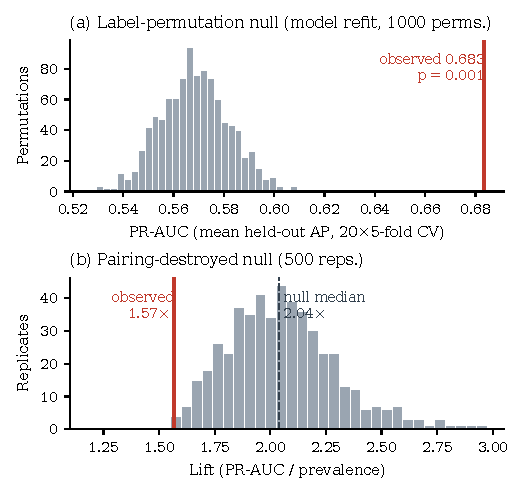
\includegraphics[width=\columnwidth]{figures/case1_nulls.pdf}
\caption{Case 1, original design. (a) The historical permutation diagnostic
(training labels permuted inside each fold, model refitted; calibration not
verified), which returned $p=0.001$. (b) Pairing-destroyed null of lift,
computed with the unfitted scorer (median 2.04$\times$; refitting the full
model on each shuffle gives a median of 1.99$\times$): the model does not
clear it. This null is conservative, so failing to clear it means only that
no response beyond regression to the mean has been shown, not that none
exists.}
\label{fig:case1}
\end{figure}

\subsection{Simulation: More Data, More Confident Rejections}
\label{sec:simresults}
Two simulation results surprised us more than the original error
(Fig.~\ref{fig:sim}). First, with no forecastable response and $r=0.25$,
raw-change label permutation rejected independence in 26\% of datasets at
$n=50$ and in 100\% at $n=500$. Each rejection was correct about
independence and wrong as evidence of a forecast: a larger sample estimates
the coupling more precisely; it does not remove it. Second, per-marker
residualisation, regressing each marker's change on its own baseline only,
the correction applied in the corrected version of our analysis, still
rejected in 8--29\% of null datasets across settings, because correlated
markers carry each other's baselines. Joint residualisation brought the rate
to 5--8\%, slightly above the nominal 5\%. A correction is a check too, and
it needs its own check.

\begin{figure*}[t]
\centering
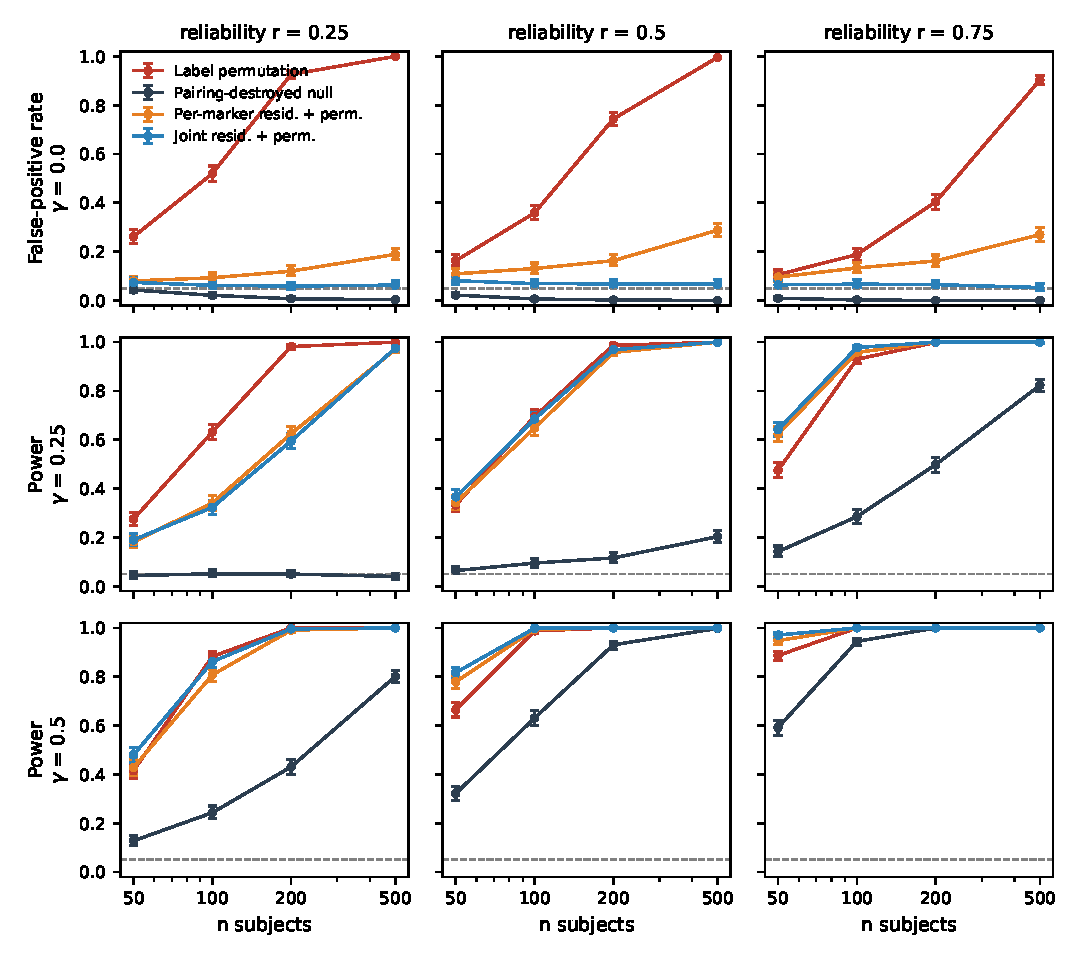
\includegraphics[width=0.85\textwidth]{figures/sim_rejection.pdf}
\caption{Simulated rejection rate against the number of subjects, 1{,}000
datasets per point; error bars are 95\% Wilson intervals for the rejection
proportions. Rows vary the strength of forecastable response
($\gamma=0$, 0.25 and 0.5); columns vary measurement reliability $r$. With
$\gamma=0$ there is no forecastable individual response, so every rejection
in the top row (labelled false-positive rate) is a false signal of
forecasting skill, even where it correctly rejects independence. On raw
change, label permutation (whole-vector) rises towards 100\% as $n$ grows;
per-marker residualisation also rises; joint residualisation stays at
5--8\%. The lower rows show power when a forecastable response exists.
Dashed line: $\alpha=0.05$.}
\label{fig:sim}
\end{figure*}

\subsection{Replication on a Second Cohort}
In MTBLS881, on raw change scores the permutation diagnostic gave $p=0.007$
at both sites. Neither site demonstrated an improvement over the
learn-nothing scorer; the 95\% interval for the model--scorer gap included
zero at both sites ($-0.037$ $[-0.231, +0.118]$ at the left atrium and
$+0.013$ $[-0.111, +0.154]$ at the pulmonary artery). The two sites come
from the same patients, so they are correlated observations, not two
replications, and their $p$-values come from the same uncalibrated per-fold
procedure, here with an unconstrained model. Whether any real signal
remains after joint residualisation, 47 patients could not tell.

\subsection{Case 2: The Explanation That Was Faithful to the Wrong Thing}
\label{sec:case2}

\emph{What we believed.} A classifier separating preoperative from
twelve-month samples (PR-AUC 0.973, CV grouped by patient) relied on
metabolites that tell us how surgery changes metabolism, and ROAR confirmed
which ones.

\emph{Why the check passed.} Removing the SHAP-ranked features one at a time
and retraining hurt the model more than removing random features, from the
third removal on; these exploratory removal results suggest that the model
relied on those features. But the first five removed included dimethyl
sulfone, isopropanol and methanol. Isopropanol is used for skin preparation,
and handling during collection can introduce exogenous compounds into
samples \cite{bernini2011, vandersar2015}; these sources describe the
general risk, not contamination of this cohort. Dimethyl sulfone is a normal
plasma metabolite that comes from diet, gut bacteria and the body's own
sulfur metabolism \cite{engelke2005}, any of which could differ before and
after surgery. We therefore treat the three as compounds of \emph{uncertain
provenance}: they may reflect biology, sample handling, or both, and an
exogenous origin would not by itself imply contamination during handling.
The deposited data cannot settle this, and the argument below does not
depend on it.

\emph{What we found.} Removing these three gave PR-AUC 0.954; removing three
established metabolites gave 0.959. Both removals reduced performance below
almost all random removals; the observed gap was 0.0056, against a
fold-to-fold standard deviation of about 0.03, and we performed no formal
equivalence test. ROAR, in other words, gave no sign of any difference in
provenance between the two groups. With the synthetic artefact feature at an
effect size similar to dimethyl sulfone's, SHAP ranked it first in 6 of 10
draws and second in the rest, and its median single-removal drop exceeded
that of every real metabolite. One caveat applies: SHAP rankings were
computed on all 177 samples, including those later used for evaluation, so
the informed removals are subject to selection bias of unquantified
magnitude \cite{varma2006}. We therefore treat the ROAR comparisons as
exploratory; the synthetic feature supports the conceptual point without
them.

\emph{The lesson.} A faithfulness test checks whether the features an
explanation ranks highly are the ones that drive the model's predictions; it
does not certify the model as a whole. Removal-based faithfulness tests
measure how much non-redundant signal a feature carries, whatever its
source. It is faithful to the model, and the
model is faithful to whatever separates the classes
\cite{adebayo2018, kumar2020}. ROAR cannot adjudicate provenance: it cannot
tell us whether the top features reflect biology, handling, or both, and for
these three compounds the question stays open.

\subsection{Case 3: The Cohort That Was Two Studies}
\label{sec:case3}

\emph{What we believed.} Urine NMR spectra separate people with type 2
diabetes from controls with PR-AUC 0.976, under CV grouped by subject.

\emph{Why the check passed.} Grouping by subject stops the model from
recognising a person it has already seen. It cannot detect a difference
shared by every member of a class.

\emph{What we found.} The 0.976 came from one random seed; over 20 seeds the
mean was 0.911 (range 0.845--0.975). We then cross-tabulated the label
against all 64 columns of the deposited metadata. Fifty-six were constant,
and apart from per-sample identifiers only sex and the label varied; no
column recorded a date, batch or run order. The deposited protocol, however,
described two different studies: 12 volunteers aged 18--55 sampled at seven
fixed times, and patients aged 30--65 with higher body-mass index sampled
one to three times. Every control sample name began with \texttt{ADG19007u}
and every patient sample name with \texttt{ADG10003u}. Cohort membership,
and with it the sampling schedule and any difference in how the two studies
collected and stored urine, is therefore perfectly confounded with the
label. Age and body-mass index were recruited under different but
overlapping ranges, so they are potential confounders as well; neither is
recorded per sample.

One methodological limit of our own audit belongs here. Which samples come
from which patient is not deposited, so we grouped patient samples with a
numbering heuristic. It merged at least three pairs of distinct patients,
which is conservative for those pairs, but we cannot rule out that it also
split one patient's samples across groups. Grouping does change the score:
over the same 20 seeds, grouped CV gave 0.911 (0.906 under an alternative,
protocol-consistent grouping) and ungrouped CV 0.969. The protocol problem,
however, does not depend on grouping: it is a property of the study design,
and no choice of folds can remove it.

\emph{The lesson.} The classifier may have learned diabetes, collection
protocol, or both; these data cannot tell which, because each protocol
contains only one class \cite{leek2010}. Because these data cannot separate
disease from collection protocol, whether the classifier's performance
reflects a difference in disease remains undetermined.

\subsection{Case 4: The Label That Was Named for Something Else}
\label{sec:case4}

\emph{What we believed.} Serum NMR separates obese from non-obese people with
ROC-AUC 0.973, the AUC of the mean ROC curve over a single stratified 5-fold
split (0.974 when we re-ran it).

\emph{Why the check passed.} When we repeated the evaluation 10 times with
the original model, CV grouped by patient and ungrouped CV both gave a mean
fold ROC-AUC of 0.965 (a different summary from the mean-curve AUC; the
re-run split's mean fold AUC was 0.976), although in ungrouped CV 65\% of
test samples had the same patient's other visit in the training folds.
Removing that leakage did not lower the score, and the agreement looked
reassuring.

\emph{What we found.} The ``non-obese'' class was the twelve-month
post-surgery visit of the same cohort. Of the 106 patients, 71 appear in both
classes and supply 80\% of the samples. The metadata record no body-mass
index, so we cannot check whether any twelve-month patient was non-obese.
The score reflects whatever differs between a person before bariatric
surgery and the same person a year later: weight loss, but potentially also
diet, supplements and medication after surgery, and a year's difference in
sample storage. These data cannot attribute it to obesity.

\emph{The lesson.} The correct name is ``pre- vs.\ post-surgery
classification.''

\subsection{Common Pattern Across the Four Cases}
In each case, the check indicated that the data contained predictive
structure, with the caveats already noted for our permutation procedure and
the exploratory ROAR comparisons. What it could not establish was where that
structure came from: from the arithmetic of the outcome, from compounds of
uncertain origin, from the collection protocol, or from surgery. Each of
these rivals would pass the check as easily as the biology we had in mind,
so passing could not distinguish them. Three habits made this easy to miss.

\emph{We reported checks, not rivals.} A methods section lists the checks
that were run. It rarely lists the alternative explanations those checks
were meant to address. Once a check is listed, it reads as a general
certificate of validity, though it addresses only one failure mode.

\emph{We trusted bigger numbers more.} A smaller $p$-value, a larger $n$, or
an AUC near 1 feels like stronger evidence. Case~1 and the simulation show a
setting in which more data produced a more confident but equally
uninformative rejection, and Case~3 one in which a high, seed-dependent
score sat on top of a design confound. In small cohorts, a score close to 1
is a reason to look for a proxy, not a reason to stop.

\emph{We checked the model, not the label.} All our checks took the label as
given. Two of our four failures were in the label itself (Cases~1 and 4),
and a third (Case~3) was in how its classes were collected. No amount of
model validation reaches a problem that sits upstream of the model.

% ===========================================================================
\section{Conclusion}
\label{sec:conclusion}

Each of our four analyses produced a result we treated as validated, and in
each the biological interpretation we attached to it was unsupported or
unidentifiable. The responder forecast shows no evidence of improvement over
an unfitted score at $n=71$; this is absence of evidence, not evidence that
no forecast is possible. The exploratory ROAR results suggest which features
the model relies on, not where those features come from. For the diabetes
classifier, these data cannot show whether its performance reflects disease
or collection protocol. The obesity classifier is a pre- vs.\ post-surgery
classifier. A check that passes addresses one failure mode under its own
assumptions; it does not establish that the interpretation is right.

These conclusions have limits. We audited our own analyses of three small
public datasets, chosen because their problems can be verified from the
published files, and we make no claim about how common these failures are in
the literature. Our findings concern validation practice and say nothing for
or against the biology of obesity, bariatric surgery or diabetes. We have
not shown that any classifier used \emph{only} an artefact; we have shown
that the checks could not rule the artefact out. The provenance of the three
compounds in Case~2 is not established. The permutation $p$-values in
Case~1 and its replication come from a per-fold procedure whose calibration
we have not verified. The simulation uses Gaussian data, a linear model and
one outcome rule, and the joint residualisation it supports also removes any
true dependence of change on baseline. The checks we discuss can be useful
when matched to their assumptions and target; our point is that passing
them is not sufficient for a biological interpretation.

% ===========================================================================
\section{Future Directions}
\label{sec:future}

For future small-$n$ metabolomics studies, including our own, we recommend
naming the rival explanations for a headline score before choosing the
tests, and asking six questions; the companion paper gives reference code
for each \cite{vyw}.

\begin{enumerate}
  \item \emph{Is the outcome computed from the features?} If so, a label
        permutation is not evidence of a forecast. If the scientific target
        is change beyond what baseline predicts, regress change on
        \emph{all} baselines inside each training fold; if baseline-dependent
        change is itself of interest, this correction removes it, and the
        question may require repeated baseline measurements or another
        design that separates measurement error from response. In either
        case, report a pairing-destroyed null as a one-sided diagnostic.
  \item \emph{Was the model refitted inside every permutation, and is the
        permutation scheme stated?} If the observed statistic sits below
        the whole null, audit the null construction, the scoring pipeline,
        the model constraints and the fitting procedure before reading the
        $p$-value.
  \item \emph{Does the model beat a score that learns nothing?} Report the
        gap with an interval that resamples subjects.
  \item \emph{Could any feature come from sample handling or drugs?} Report
        results with and without such features, and run a feature known to
        carry no biology through the attribution pipeline.
  \item \emph{Does any metadata column or collection protocol line up with
        the label?} Cross-tabulate the label against every column and read
        how each class was collected.
  \item \emph{What, in one sentence, physically distinguishes the two
        classes?} If the sentence differs from the title, change the title.
\end{enumerate}

These questions can be asked of the existing records, although resolving
some of the problems they reveal requires new measurements or a different
study design. For the present audit, four analyses would strengthen the
evidence: rerunning the Case~1 raw-change test with whole-vector
permutations, to assess how sensitive the conclusion is to the permutation
scheme; estimating the rejection rate of the per-fold scheme on repeated
simulated data under the null hypothesis it is meant to test, to check its
calibration (keeping ``no forecastable response'' distinct from
``features and label are independent,'' which are not the same condition);
computing the Case~2 SHAP rankings inside each training fold; and repeating
Case~4 in a cohort with recorded body-mass index and lean controls.

% ===========================================================================
\section*{Data and Code Availability}
MTBLS242, MTBLS1 and MTBLS881 are public through MetaboLights \cite{haug2020}.
The analysis code, the simulation and a record of every reported number with
its script and random seed are available from the authors.

\section*{Acknowledgment}
The authors thank Asst.\ Prof.\ Dr.\ Nont Kanungsukkasem, School of
Information Technology, King Mongkut's Institute of Technology Ladkrabang, for
advising this work. This research received no specific funding.

% ===========================================================================
\begin{thebibliography}{00}
\bibitem{vyw} C. Orrudee and K. C. Shomwiwat, ``Validated, yet wrong: Four ways small-$n$ metabolomics machine learning passes standard checks,'' unpublished draft, 2026.
\bibitem{ojala2010} M. Ojala and G. C. Garriga, ``Permutation tests for studying classifier performance,'' \textit{J. Mach. Learn. Res.}, vol. 11, pp. 1833--1863, 2010.
\bibitem{hooker2019} S. Hooker, D. Erhan, P.-J. Kindermans, and B. Kim, ``A benchmark for interpretability methods in deep neural networks,'' in \textit{Proc. Adv. Neural Inf. Process. Syst. (NeurIPS)}, vol. 32, 2019.
\bibitem{oldham1962} P. D. Oldham, ``A note on the analysis of repeated measurements of the same subjects,'' \textit{J. Chronic Dis.}, vol. 15, no. 10, pp. 969--977, 1962, doi: 10.1016/0021-9681(62)90116-9.
\bibitem{barnett2005} A. G. Barnett, J. C. van der Pols, and A. J. Dobson, ``Regression to the mean: what it is and how to deal with it,'' \textit{Int. J. Epidemiol.}, vol. 34, no. 1, pp. 215--220, Feb. 2005, doi: 10.1093/ije/dyh299.
\bibitem{tu2007} Y.-K. Tu and M. S. Gilthorpe, ``Revisiting the relation between change and initial value: a review and evaluation,'' \textit{Stat. Med.}, vol. 26, no. 2, pp. 443--457, Jan. 2007, doi: 10.1002/sim.2538.
\bibitem{archie1981} J. P. Archie, ``Mathematic coupling of data: a common source of error,'' \textit{Ann. Surg.}, vol. 193, no. 3, pp. 296--303, Mar. 1981, doi: 10.1097/00000658-198103000-00008.
\bibitem{leek2010} J. T. Leek \textit{et al.}, ``Tackling the widespread and critical impact of batch effects in high-throughput data,'' \textit{Nat. Rev. Genet.}, vol. 11, no. 10, pp. 733--739, Oct. 2010, doi: 10.1038/nrg2825.
\bibitem{han2022} W. Han and L. Li, ``Evaluating and minimizing batch effects in metabolomics,'' \textit{Mass Spectrom. Rev.}, vol. 41, no. 3, pp. 421--442, 2022, doi: 10.1002/mas.21672.
\bibitem{bernini2011} P. Bernini, I. Bertini, C. Luchinat, P. Nincheri, S. Staderini, and P. Turano, ``Standard operating procedures for pre-analytical handling of blood and urine for metabolomic studies and biobanks,'' \textit{J. Biomol. NMR}, vol. 49, no. 3--4, pp. 231--243, 2011, doi: 10.1007/s10858-011-9489-1.
\bibitem{vandersar2015} S. A. van der Sar \textit{et al.}, ``Ethanol contamination of cerebrospinal fluid during standardized sampling and its effect on $^1$H-NMR metabolomics,'' \textit{Anal. Bioanal. Chem.}, vol. 407, no. 16, pp. 4835--4839, Jun. 2015, doi: 10.1007/s00216-015-8663-9.
\bibitem{kapoor2023} S. Kapoor and A. Narayanan, ``Leakage and the reproducibility crisis in machine-learning-based science,'' \textit{Patterns}, vol. 4, no. 9, Art. no. 100804, Sep. 2023, doi: 10.1016/j.patter.2023.100804.
\bibitem{collins2024} G. S. Collins \textit{et al.}, ``TRIPOD+AI statement: updated guidance for reporting clinical prediction models that use regression or machine learning methods,'' \textit{BMJ}, vol. 385, Art. no. e078378, 2024, doi: 10.1136/bmj-2023-078378.
\bibitem{haug2020} K. Haug \textit{et al.}, ``MetaboLights: a resource evolving in response to the needs of its scientific community,'' \textit{Nucleic Acids Res.}, vol. 48, no. D1, pp. D440--D444, Jan. 2020, doi: 10.1093/nar/gkz1019.
\bibitem{mtbls242} EMBL-EBI, ``MetaboLights study MTBLS242: Metabolomic fingerprint of severe obesity is dynamically affected by bariatric surgery in a procedure-dependent manner,'' dataset. [Online]. Available: \url{https://www.ebi.ac.uk/metabolights/MTBLS242}
\bibitem{gralka2015} E. Gralka, C. Luchinat, L. Tenori, B. Ernst, M. Thurnheer, and B. Schultes, ``Metabolomic fingerprint of severe obesity is dynamically affected by bariatric surgery in a procedure-dependent manner,'' \textit{Am. J. Clin. Nutr.}, vol. 102, no. 6, pp. 1313--1322, Dec. 2015, doi: 10.3945/ajcn.115.110536.
\bibitem{salek2007} R. M. Salek \textit{et al.}, ``A metabolomic comparison of urinary changes in type 2 diabetes in mouse, rat, and human,'' \textit{Physiol. Genomics}, vol. 29, no. 2, pp. 99--108, Apr. 2007, doi: 10.1152/physiolgenomics.00194.2006.
\bibitem{maltesen2020} R. G. Maltesen, R. Wimmer, and B. S. Rasmussen, ``A longitudinal serum NMR-based metabolomics dataset of ischemia-reperfusion injury in adult cardiac surgery,'' \textit{Sci. Data}, vol. 7, Art. no. 198, 2020, doi: 10.1038/s41597-020-0545-0.
\bibitem{engelke2005} U. F. H. Engelke, A. Tangerman, M. A. A. P. Willemsen, D. Moskau, S. Loss, S. H. Mudd, and R. A. Wevers, ``Dimethyl sulfone in human cerebrospinal fluid and blood plasma confirmed by one-dimensional $^1$H and two-dimensional $^1$H--$^{13}$C NMR,'' \textit{NMR Biomed.}, vol. 18, no. 5, pp. 331--336, 2005, doi: 10.1002/nbm.966.
\bibitem{varma2006} S. Varma and R. Simon, ``Bias in error estimation when using cross-validation for model selection,'' \textit{BMC Bioinformatics}, vol. 7, Art. no. 91, 2006, doi: 10.1186/1471-2105-7-91.
\bibitem{adebayo2018} J. Adebayo, J. Gilmer, M. Muelly, I. Goodfellow, M. Hardt, and B. Kim, ``Sanity checks for saliency maps,'' in \textit{Proc. Adv. Neural Inf. Process. Syst. (NeurIPS)}, vol. 31, 2018.
\bibitem{kumar2020} I. E. Kumar, S. Venkatasubramanian, C. Scheidegger, and S. Friedler, ``Problems with Shapley-value-based explanations as feature importance measures,'' in \textit{Proc. 37th Int. Conf. Mach. Learn. (ICML)}, PMLR vol. 119, 2020, pp. 5491--5500.
\end{thebibliography}

\end{document}
